\section{Příklad 1}
% Jako parametr zadejte skupinu (A-H)
\prvniZadani{C}

Převedeme trojúhlník na hvězdu:
    \begin{figure}[h]
		\begin{center}
			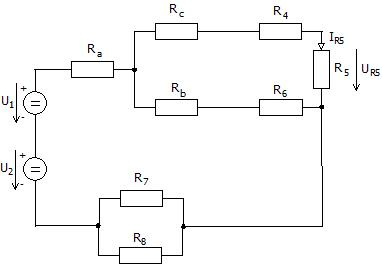
\includegraphics[width=8cm,keepaspectratio]{fig/Pr1_1_2019.jpeg}
		\end{center}
	\end{figure}
	\begin{eqnarray*}
        R_{a} &= & \frac{R_{1} * R_{2}}{R_{1} + R_{2} + R_{3}} = \frac{450 * 810}{450 + 810 + 190} = 251.3793 \Omega\\
        R_{b} &= & \frac{R_{2} * R_{3}}{R_{1} + R_{2} + R_{3}} = \frac{810 * 190}{450 + 810 + 190} = 106.1379 \Omega\\
        R_{c} &= & \frac{R_{3} * R_{1}}{R_{1} + R_{2} + R_{3}} = \frac{190 * 450}{450 + 810 + 190} = 58.9655 \Omega\\
	\end{eqnarray*}

Zjednodušíme zapojení:
    \begin{eqnarray*}
        U_{12} &= & U_{1} + U_{2} = 100 + 80 = 180 V\\
		R_{78} &= & \frac{R_{7} * R_{8}}{R_{7} + R_{8}} = \frac{260 * 180}{260 + 180} = 106.3634 \Omega\\
		R_{45c} &= & R_{4} + R_{5} + R_{c} = 220 + 220 + 58.9655 = 498.9655 \Omega\\
		R_{6b} &= & R_{6} + R_{b} = 720 + 106.1379 = 826.1379 \Omega\\
		R_{456cb} &= & \frac{R_{45c} * R_{6b}}{R_{45c} + R_{6b}} = \frac{498.9655 * 826.1379}{498.9655 + 826.1379} = 311.0809 \Omega\\
		R_{45678abc} &= & R_{a} + R_{456cb} + R_{78} = 251.3793 + 311.0809 + 106.3634 = 668.8236 \Omega\\
	\end{eqnarray*}

Vypočítáme proud:
    \begin{eqnarray*}
        I &= & \frac{U_{12}}{R_{45678abc}} = \frac{180}{668.8236} = 0.2691 A\\
	\end{eqnarray*}

Vypočítáme hledané hodnoty:
    \begin{eqnarray*}
        U_{456bc} &= & I * R_{456bc} = 0.2691 * 311.0809 = 83.7119 V\\
        I_{R5} &= & \frac{U_{456bc}}{R_{45c}} = \frac{83.7119}{498.9655} = 0.1678 A\\
        U_{R5} &= & I_{R5} * R_{R5} = 0.1678 * 220 = 36.9160 V\\
	\end{eqnarray*}

Hledané hodnoty $U_{R5}$ a $I_{R5}$ jsou:
    \begin{eqnarray*}
        U_{R5} &= & 36.9160 V\\
        I_{R5} &= & 0.1678 A\\
	\end{eqnarray*}